% Procedencia (nunca se imprime): véase sources/outline_sources.md (año 3:
% firmas espectrales; sensores ópticos, térmicos y de radar; interferometría
% radar; modelos digitales de elevaciones; operaciones de SIG).
% Resumen: sources/book5/BRIEFS.md, cap. 25. Curvas de figdata/bachelor-3/
% spectral_signatures.py (espectros de ECOSTRESS y bandas OLI de Landsat 8),
% thermal_ir.py (ley de Planck, temperaturas de brillo y un píxel mixto),
% insar_mogi.py (el interferograma envuelto de una fuente de Mogi) y
% varden_gis.py (pendiente, orientación y una superposición en las colinas de
% Varden, desde figdata/shared/region.py, solo lectura). Valores de ejercicios
% y problemas en la calculadora auxiliar del libro 5 calc/ch25.py. El monte Halvren, sus coladas
% y sus fumarolas son inventados. La superposición del resumen (pendiente > 15 grados sobre
% caliza a menos de 200 m del río) está vacía en el modelo de Varden: el
% fondo del valle es plano; la superposición impresa usa la lutita a menos de 1 km.
\chapter{Teledetección y SIG}\label{ch:b3:remote-sensing-gis}

En 1997 el terreno de una zona salvaje de la cordillera de las Cascadas, cerca del conjunto de
volcanes llamado las Tres Hermanas, empezó a elevarse. En 2001 su centro estaba
\qty{15}{cm} más alto. No hay ningún volcán directamente sobre el abombamiento, y la
última erupción de la zona había ocurrido hace 1500 años. El levantamiento no lo detectó
nadie caminando sobre él: apareció como una diana de anillos de colores cuando se
combinaron imágenes de radar de la región, tomadas desde órbita con años de diferencia.
Los anillos situaban el magma intrusivo a entre 6 y \qty{7}{km} de profundidad; en marzo de 2004
un enjambre de más de 300 terremotos pequeños se produjo junto a su centro.
Este capítulo explica cómo un satélite mide un cambio de unos pocos
centímetros desde cientos de kilómetros de altura, qué ven del terreno los demás
sensores en órbita y cómo se combinan los mapas que producen en un
sistema de información geográfica.
% ledger: usgs:insar-fs

\begin{recall}
El espectro electromagnético, la ley de Planck del cuerpo negro, la emisividad
y la ley de Kirchhoff, la reflectancia y la interferencia de ondas están en los
libros de física. La teledetección, las imágenes de satélite, las proyecciones
cartográficas y el posicionamiento por satélite están en los libros del colegio.
Las ventanas atmosféricas y las bandas fotométricas están en el volumen de primer
año, en su capítulo sobre telescopios; el modelo digital de elevaciones y el sistema
de información geográfica que lo almacena, en su capítulo sobre mapas geológicos; el
primer mapa radar del desplazamiento de un terremoto, en su capítulo sobre la fuente
sísmica. La fuente de Mogi de una cámara magmática que se hincha está en el volumen
de segundo año, en su capítulo sobre erupciones volcánicas.
\end{recall}

\section{Firmas espectrales y sensores ópticos}\label{sec:b3:remote-sensing-gis:optical}

La luz solar que llega al terreno se absorbe en parte y en parte se refleja,
en proporciones que dependen de la longitud de onda y de lo que esté hecho el
terreno. Un sensor en órbita mide la luz reflejada en unos pocos intervalos de
longitud de onda, sus bandas, y las razones entre las bandas identifican la
superficie.

\begin{definition}[Firma espectral]\label{def:b3:remote-sensing-gis:signature}
La \emph{firma espectral}\index{firma espectral} de un material es
su reflectancia en función de la longitud de onda, $R(\lambda)$, la fracción de
la radiación incidente que refleja. En el infrarrojo térmico, donde
las superficies emiten en lugar de reflejar, la firma es la emisividad
$\varepsilon(\lambda)$; para una muestra opaca $\varepsilon = 1 - R$.
\end{definition}

\begin{omfigure}
\centering
\begin{tikzpicture}
\begin{axis}[width=0.9\linewidth, height=6.4cm, xmin=0.4, xmax=2.5, ymin=0, ymax=1,
  xlabel={longitud de onda (\unit{\micro\metre})}, ylabel={reflectancia},
  tick label style={font=\scriptsize}, label style={font=\small},
  legend style={font=\scriptsize, at={(0.5,-0.24)}, anchor=north, /tikz/every even column/.append style={column sep=4pt}},
  legend columns=5, clip=false]
\fill[black!8] (axis cs:0.45,0) rectangle (axis cs:0.51,1);
\fill[black!8] (axis cs:0.53,0) rectangle (axis cs:0.59,1);
\fill[black!8] (axis cs:0.64,0) rectangle (axis cs:0.67,1);
\fill[black!8] (axis cs:0.85,0) rectangle (axis cs:0.88,1);
\fill[black!8] (axis cs:1.57,0) rectangle (axis cs:1.65,1);
\fill[black!8] (axis cs:2.11,0) rectangle (axis cs:2.29,1);
\addplot[very thick, green!50!black] table[x=um, y=grass] {figdata/out/bachelor-3-spectral_signatures-spectra.dat};
\addlegendentry{hierba verde}
\addplot[thick, brown!70!black, dashed] table[x=um, y=soil] {figdata/out/bachelor-3-spectral_signatures-spectra.dat};
\addlegendentry{arena marrón}
\addplot[thick, black!55] table[x=um, y=kaol] {figdata/out/bachelor-3-spectral_signatures-spectra.dat};
\addlegendentry{caolinita}
\addplot[thick, red!70!black, dash dot] table[x=um, y=hem] {figdata/out/bachelor-3-spectral_signatures-spectra.dat};
\addlegendentry{hematites}
\addplot[thick, omDef] table[x=um, y=water] {figdata/out/bachelor-3-spectral_signatures-spectra.dat};
\addlegendentry{agua}
\node[font=\tiny, anchor=south] at (axis cs:0.48,1) {2};
\node[font=\tiny, anchor=south] at (axis cs:0.56,1) {3};
\node[font=\tiny, anchor=south] at (axis cs:0.655,1) {4};
\node[font=\tiny, anchor=south] at (axis cs:0.865,1) {5};
\node[font=\tiny, anchor=south] at (axis cs:1.61,1) {6};
\node[font=\tiny, anchor=south] at (axis cs:2.2,1) {7};
\end{axis}
\end{tikzpicture}
\par\smallskip{\small Espectros de reflectancia de laboratorio de cinco superficies (ECOSTRESS
Spectral Library, reproducidos por cortesía del Jet Propulsion
Laboratory, California Institute of Technology), con las seis bandas reflectivas
2 a 7 del sensor Landsat~8 y 9 sombreadas. La hierba verde es oscura en el
visible y la más brillante en el infrarrojo cercano; la caolinita es brillante en todo el
espectro salvo por una estrecha absorción en \qty{2.2}{\micro\metre}; la hematites absorbe
el azul y el verde y refleja el rojo; el agua refleja unos pocos por ciento en
cada longitud de onda.}\label{fig:b3:remote-sensing-gis:spectra}
\end{omfigure}
% ledger: data:b5-ecostress, usgs:landsat8-bands, nasa:ndvi

Las firmas de la figura anterior son el vocabulario de la teledetección
óptica. La clorofila de las hojas absorbe con fuerza entre 0.4 y
\qty{0.7}{\micro\metre}, para la fotosíntesis, mientras que las células de las hojas
reflejan con fuerza entre 0.7 y \qty{1.1}{\micro\metre}: la hierba verde refleja un
\qty{5}{\percent} de la luz roja de la banda~4 y un \qty{50}{\percent} del infrarrojo
cercano de la banda~5, un salto que ninguna roca ni suelo presenta. Más allá, dos
depresiones profundas cerca de 1.4 y \qty{1.9}{\micro\metre} son donde el agua
líquida absorbe. La arena marrón se aclara de forma constante hacia el infrarrojo.
La caolinita, una arcilla, es blanca en el visible y tiene una absorción estrecha en
\qty{2.20}{\micro\metre}, dentro de la banda~7, lo que la hace más oscura allí que
en la banda~6; un \omterm{def:b3:remote-sensing-gis:sensors}{sensor hiperespectral} resuelve su forma y permite distinguir una arcilla
de otra. La hematites absorbe el azul y el verde: de ahí su color rojo.
% ledger: nasa:ndvi, data:b5-ecostress

\begin{definition}[Resolución espacial, espectral y radiométrica; tiempo de revisita]\label{def:b3:remote-sensing-gis:resolutions}
La \emph{resolución espacial}\index{resolución espacial} de una imagen es el
tamaño sobre el terreno de uno de sus píxeles. Su \emph{resolución
espectral}\index{resolución espectral} es el número y la anchura de sus
bandas, y su \emph{resolución radiométrica}\index{resolución radiométrica} es el
número de niveles en que se registra cada medida, $2^b$ para $b$ bits.
El \emph{tiempo de revisita}\index{tiempo de revisita} de un satélite es el intervalo
entre dos de sus observaciones de un mismo lugar.
\end{definition}

Las cuatro no pueden ser finas a la vez: los píxeles más pequeños y las bandas más estrechas
recogen cada una menos luz, y una franja estrecha tarda más en cubrir la
Tierra. El instrumento de imagen de Landsat~8, lanzado en 2013, tiene nueve bandas, la mayoría de
ellas con píxeles de \qty{30}{m} y una banda pancromática de \qty{15}{m}; el
instrumento registra 4096 niveles (12 bits), frente a los instrumentos de Landsat 1 a 7
que registraban 256. Desde una órbita heliosíncrona a \qty{705}{km} de altura
toma imágenes de una franja de \qty{185}{km} de ancho y vuelve sobre el mismo terreno cada 16~días;
Landsat~9, en la misma órbita y desfasado 8~días, reduce a la mitad la espera.
El instrumento multiespectral de cada satélite Sentinel-2 tiene 13 bandas, de 10, 20
o \qty{60}{m}, sobre una franja de \qty{290}{km}; con dos satélites en la
misma órbita, el \omterm{def:b3:remote-sensing-gis:resolutions}{tiempo de revisita} en el Ecuador es de 5~días.
% ledger: usgs:landsat8-bands, usgs:landsat8-orbit, esa:s2-msi, esa:s2-orbit

\begin{definition}[Sensores multiespectrales e hiperespectrales]\label{def:b3:remote-sensing-gis:sensors}
Un \emph{sensor multiespectral}\index{sensor multiespectral} registra de pocas
a unas pocas decenas de bandas, separadas por huecos. Un \emph{sensor
hiperespectral}\index{sensor hiperespectral} registra muchas bandas estrechas y contiguas,
de modo que cada píxel lleva un espectro casi continuo que puede
compararse con una biblioteca espectral como la de la figura anterior.
\end{definition}

Entre el terreno y el sensor se encuentra la atmósfera. Esta dispersa
hacia el sensor luz solar que nunca tocó el terreno, sobre todo a
longitudes de onda cortas, la radiancia de trayectoria, y absorbe parte de lo que el
terreno refleja fuera de las ventanas atmosféricas.

\begin{definition}[Corrección atmosférica]\label{def:b3:remote-sensing-gis:atm-correction}
La \emph{corrección atmosférica}\index{corrección atmosférica} es la
conversión de la radiancia medida en el tope de la atmósfera en la
reflectancia de la superficie, eliminando la radiancia de trayectoria y compensando
la absorción a lo largo de los dos trayectos de la luz, de bajada y de subida.
\end{definition}

La corrección más sencilla resta en cada banda el valor de los píxeles más
oscuros de la escena, agua profunda y limpia o una sombra, que deberían reflejar
casi nada: lo que muestran es la radiancia de trayectoria. Las correcciones cuidadosas
modelizan las moléculas, los aerosoles y el vapor de agua de la atmósfera.

\begin{definition}[Índice de vegetación de diferencia normalizada]\label{def:b3:remote-sensing-gis:ndvi}
El \emph{índice de vegetación de diferencia
normalizada}\index{indice de vegetación de diferencia normalizada@índice de vegetación de diferencia normalizada} (NDVI) de un píxel es
\[
\mathrm{NDVI} = \frac{R_\mathrm{NIR} - R_\mathrm{red}}{R_\mathrm{NIR} + R_\mathrm{red}} ,
\]
calculado a partir de sus reflectancias en una banda del infrarrojo cercano y en una banda roja.
\end{definition}

El índice se sitúa entre $-1$ y $+1$. El terreno sin hojas verdes da un
valor cercano a cero: roca desnuda, arena o nieve \num{0.1} o menos,
matorrales y pastizales de 0.2 a 0.3, selvas templadas y tropicales de 0.6 a
0.8; las hojas verdes más densas se acercan a 0.8 o 0.9. A partir de los espectros de la
figura anterior, a través de las bandas 4 y 5, la hierba da 0.82, la arena marrón
0.15 y el agua $-0.01$. Al ser una razón, el índice no cambia cuando
ambas bandas se atenúan en la misma proporción, por una pendiente orientada de espaldas
a la luz o por una neblina fina y uniforme: mide la vegetación, no la
iluminación. Una radiancia de trayectoria aditiva, mayor en el rojo, sí lo altera,
por eso el índice se calcula a partir de reflectancias corregidas
(el \cref{exo:b3:remote-sensing-gis:12}).
% ledger: nasa:ndvi, data:b5-ecostress

\section{El infrarrojo térmico}\label{sec:b3:remote-sensing-gis:thermal}

A las temperaturas del terreno, en torno a \qty{300}{K}, la ley de Planck sitúa
el máximo de emisión de un cuerpo negro cerca de \qty{9.7}{\micro\metre}, en la
ventana atmosférica del infrarrojo térmico. Allí el sensor mide lo que
la superficie emite, no lo que refleja. El sensor térmico de Landsat~8
tiene dos bandas, de 10.6 a 11.19 y de 11.5 a \qty{12.51}{\micro\metre}, con
píxeles de \qty{100}{m}.
% ledger: const:h, const:c, const:kB, usgs:landsat8-bands

\begin{definition}[Temperatura de brillo]\label{def:b3:remote-sensing-gis:brightness}
La \emph{temperatura de brillo}\index{temperatura de brillo} $T_b$ de una
superficie a la longitud de onda $\lambda$ es la temperatura del cuerpo negro
que emitiría la radiancia espectral $L$ medida sobre ella a esa
longitud de onda. La \emph{temperatura cinética} es la temperatura termodinámica
de la superficie, la que leería un termómetro.
\end{definition}

\begin{proposition}[Temperatura de brillo a partir de una radiancia]\label{prop:b3:remote-sensing-gis:planck-inversion}
Con $c_1 = 2hc^2$ y $c_2 = hc/k$, una radiancia espectral $L$ a la
longitud de onda $\lambda$ tiene la \omterm{def:b3:remote-sensing-gis:brightness}{temperatura de brillo}
\[
T_b = \frac{c_2}{\lambda \ln\!\left(1 + \dfrac{c_1}{\lambda^5 L}\right)} .
\]
Una superficie de emisividad $\varepsilon < 1$ a la temperatura cinética $T$
emite $L = \varepsilon B_\lambda(T)$ y tiene $T_b < T$.
\end{proposition}

\begin{proof}
La ley de Planck da $B_\lambda(T) = c_1\lambda^{-5}/(e^{c_2/\lambda T} -
1)$. Igualando $B_\lambda(T_b) = L$ y despejando, $e^{c_2/\lambda T_b} = 1 +
c_1/(\lambda^5L)$, que es la fórmula. $B_\lambda$ crece con la
temperatura, así que $\varepsilon B_\lambda(T) < B_\lambda(T)$ implica $T_b < T$.
\end{proof}
% ledger: const:h, const:c, const:kB

La diferencia importa. En el centro de la banda~10, \qty{10.9}{\micro\metre},
una superficie a \qty{300}{K} con una emisividad de 0.95 tiene una \omterm{def:b3:remote-sensing-gis:brightness}{temperatura de brillo}
de \qty{296.6}{K}; con 0.99, de \qty{299.3}{K}: una centésima de
emisividad vale más de medio kelvin. Los espectros de laboratorio dan, en
la banda~10, una emisividad de 0.98 para la hierba, 0.99 para el agua y
0.97 para la arena marrón. Cartografiar una temperatura desde órbita requiere, por tanto,
la emisividad de cada píxel y una corrección de la emisión y de la
absorción del aire interpuesto.
% ledger: data:b5-ecostress

\begin{omfigure}
\centering
\begin{tikzpicture}
\begin{groupplot}[group style={group size=2 by 1, horizontal sep=1.5cm},
  width=0.48\linewidth, height=0.42\linewidth,
  tick label style={font=\scriptsize}, label style={font=\small}, title style={font=\small}]
\nextgroupplot[title={radiancia de cuerpo negro}, xmode=log, ymode=log, xmin=1, xmax=25,
  ymin=0.01, ymax=1e5, xlabel={longitud de onda (\unit{\micro\metre})},
  ylabel={$B_\lambda$ (\unit{W.m^{-2}.sr^{-1}.\micro\metre^{-1}})},
  xtick={1,2,5,10,20}, xticklabels={1,2,5,10,20}]
\fill[black!10] (axis cs:10.6,0.01) rectangle (axis cs:11.19,1e5);
\fill[black!10] (axis cs:2.11,0.01) rectangle (axis cs:2.29,1e5);
\addplot[thick, omDef] table[x=um, y=b300] {figdata/out/bachelor-3-thermal_ir-planck.dat};
\addplot[thick, omDef, dashed] table[x=um, y=b400] {figdata/out/bachelor-3-thermal_ir-planck.dat};
\addplot[thick, red!70!black] table[x=um, y=b1443] {figdata/out/bachelor-3-thermal_ir-planck.dat};
\node[font=\scriptsize, omDef, anchor=north east] at (axis cs:24,3) {\qty{300}{K}};
\node[font=\scriptsize, omDef, anchor=south west] at (axis cs:12.5,30) {\qty{400}{K}};
\node[font=\scriptsize, red!70!black, anchor=south west] at (axis cs:3.2,2000) {\qty{1443}{K}};
\node[font=\tiny, anchor=north] at (axis cs:10.9,1e5) {10};
\node[font=\tiny, anchor=north] at (axis cs:2.2,1e5) {7};
\nextgroupplot[title={píxel mixto, banda 10}, xmin=0, xmax=1, ymin=285, ymax=375,
  xlabel={fracción $f$ del píxel a \qty{370}{K}}, ylabel={temperatura (\unit{K})},
  legend style={font=\scriptsize, at={(0.97,0.03)}, anchor=south east}]
\addplot[thick, red!70!black] table[x=f, y=tb] {figdata/out/bachelor-3-thermal_ir-mixed.dat};
\addlegendentry{temperatura de brillo}
\addplot[thick, black!60, dashed, domain=0:1] {290 + 80*x};
\addlegendentry{temperatura media}
\end{groupplot}
\end{tikzpicture}
\par\smallskip{\small Izquierda, la ley de Planck para superficies a 300 y \qty{400}{K}
y para la lava de una erupción a \qty{1170}{\celsius} (\qty{1443}{K}), con
la banda~7 del infrarrojo de onda corta y la banda térmica~10 de Landsat~8 sombreadas.
Derecha, la \omterm{def:b3:remote-sensing-gis:brightness}{temperatura de brillo} en la banda~10 de un píxel en el que una fracción
$f$ está a \qty{370}{K} y el resto a \qty{290}{K}, frente a la
temperatura media ponderada por área: la parte caliente cuenta más de lo que
su área sugiere.}\label{fig:b3:remote-sensing-gis:thermal}
\end{omfigure}
% ledger: const:h, const:c, const:kB, usgs:landsat8-bands, usgs:kilauea-temp

La lava a \qty{1170}{\celsius} tiene su máximo cerca de \qty{2.0}{\micro\metre}: una
colada reciente mucho menor que un píxel ilumina las bandas del infrarrojo de onda corta
de un sensor óptico, de día o de noche. Un píxel rara vez es uniforme, y
la ley de Planck no es lineal en la temperatura.
% ledger: usgs:kilauea-temp

\begin{proposition}[Un píxel mixto]\label{prop:b3:remote-sensing-gis:mixed}
Un píxel del que una fracción $f$ emite como cuerpo negro a $T_h$ y el resto
a $T_0 < T_h$ tiene la radiancia $L = fB_\lambda(T_h) + (1 - f)B_\lambda(T_0)$,
y, para $0 < f < 1$, su \omterm{def:b3:remote-sensing-gis:brightness}{temperatura de brillo} supera a la
temperatura media ponderada por área $fT_h + (1 - f)T_0$.
\end{proposition}

\begin{proof}
La radiancia es la media ponderada por área de las radiancias. Escríbase $B_\lambda(T)
= c_1\lambda^{-5}g(c_2/\lambda T)$ con $g(x) = 1/(e^x - 1)$; en la
variable $T$, con $x = c_2/\lambda T$, la segunda derivada de
$g(c_2/\lambda T)$ es $(x g''(x) + 2g'(x))\,x/T^2$, positiva cuando $x(e^x + 1)
> 2(e^x - 1)$, es decir, $x > 2\tanh(x/2)$, que se cumple para todo $x > 0$:
$B_\lambda$ es convexa en $T$. Por convexidad
la media de las radiancias supera a la radiancia de la temperatura media, y
$B_\lambda$ crece con $T$, luego $T_b > fT_h + (1 - f)T_0$.
\end{proof}

Un píxel con un \qty{5}{\percent} de
suelo de fumarola a \qty{370}{K} sobre un fondo a \qty{290}{K} tiene una
temperatura media de \qty{294}{K}, pero una \omterm{def:b3:remote-sensing-gis:brightness}{temperatura de brillo} de \qty{295.3}{K};
con un \qty{10}{\percent}, \qty{300.4}{K}. Los puntos calientes destacan en una
imagen térmica, y su temperatura no puede leerse a partir de una sola banda: dos bandas
de longitud de onda distinta dan dos ecuaciones para $f$ y $T_h$.

\section{Radar y lidar}\label{sec:b3:remote-sensing-gis:radar}

Un sensor óptico o térmico es pasivo: mide la luz que envía el terreno. Un radar o un
\omterm{def:b3:remote-sensing-gis:lidar}{lidar} es activo: envía un pulso y mide el tiempo de su eco.
Las microondas atraviesan las nubes, y el radar aporta su propia iluminación,
de modo que observa de día y de noche con cualquier tiempo.
% ledger: esa:s1-sar

\begin{definition}[Radar de apertura sintética; retrodispersión de radar]\label{def:b3:remote-sensing-gis:sar}
Un \emph{radar de apertura sintética}\index{radar de apertura sintética} (SAR)
es un radar transportado a lo largo de una trayectoria que mira lateralmente, y que combina los
ecos que registra desde un mismo punto del terreno a lo largo de una longitud de su
trayectoria, conservando sus fases, como si hubieran sido recibidos por una sola antena tan
larga como esa longitud. La \emph{retrodispersión de radar}\index{retrodispersión de radar}
de una superficie es la fracción de la potencia que recibe que devuelve
hacia la antena.
\end{definition}

\begin{omfigure}
\centering
\begin{tikzpicture}[>=stealth, font=\small, x=1cm, y=1cm]
\fill[black!12] (-0.5,-0.35) rectangle (10.5,0);
\draw[thick] (-0.5,0) -- (10.5,0);
% satellite
\fill[omDef] (0.6,4.6) rectangle (1.4,5.0);
\draw[thick, omDef] (0.35,4.45) -- (1.65,5.15);
\draw (1.0,4.8) circle (0.12); \fill (1.0,4.8) circle (0.03);
\node[font=\scriptsize, anchor=south, align=center] at (1.0,5.3) {trayectoria (acimut)\\hacia dentro de la página};
% nadir
\draw[dashed, black!60] (1.0,4.4) -- (1.0,0);
\node[font=\scriptsize, anchor=north] at (1.0,-0.4) {nadir};
\draw[<->, black!60] (0.3,0) -- node[left, font=\scriptsize] {$h$} (0.3,4.4);
% beam
\fill[omDef!12] (1.0,4.4) -- (4.3,0) -- (9.6,0) -- cycle;
\draw[omDef!60] (1.0,4.4) -- (4.3,0); \draw[omDef!60] (1.0,4.4) -- (9.6,0);
\node[font=\scriptsize, anchor=north] at (4.3,-0.4) {distancia cercana};
\node[font=\scriptsize, anchor=north] at (9.6,-0.4) {distancia lejana};
\draw[<->] (4.3,-1.0) -- node[below, font=\scriptsize] {franja barrida} (9.6,-1.0);
% target and slant range
\fill[red!70!black] (7.0,0) circle (0.07);
\draw[thick, red!70!black] (1.0,4.4) -- node[above, sloped, font=\scriptsize] {distancia oblicua $R$} (7.0,0);
\draw[black!60] (7.0,0) -- (7.0,1.8);
\draw[black!60] (7.0,0.9) arc (90:126.25:0.9);
\node[font=\scriptsize] at (6.6,1.2) {$\theta$};
\draw[->, very thick, omThm] (7.0,0) -- (6.2,0.59) node[anchor=north east, font=\scriptsize, inner sep=1pt] {LOS};
\draw[<->, black!60] (1.0,-1.6) -- node[below, font=\scriptsize] {distancia en el terreno} (7.0,-1.6);
\draw[black!60] (1.0,-1.5) -- (1.0,-1.7); \draw[black!60] (7.0,-1.5) -- (7.0,-1.7);
\end{tikzpicture}
\par\smallskip{\small La geometría de un radar de visión lateral, en el plano
perpendicular a su trayectoria. El haz ilumina una franja a un lado del
nadir; un punto del terreno se ve a la distancia oblicua $R$ bajo el
ángulo de incidencia $\theta$, a lo largo de la \omterm{def:b3:remote-sensing-gis:insar}{línea de visión} (LOS). Los ecos se ordenan
por su retardo a través de la trayectoria, en distancia, y por la historia de fase
de la apertura sintética a lo largo de ella, en acimut.}\label{fig:b3:remote-sensing-gis:sar}
\end{omfigure}

\begin{proposition}[Resolución en acimut]\label{prop:b3:remote-sensing-gis:azimuth}
Una antena real de longitud $L$ a la distancia oblicua $R$ separa dos puntos del
terreno a lo largo de su trayectoria solo si distan más de unos $R\lambda/L$
entre sí. Un \omterm{def:b3:remote-sensing-gis:sar}{radar de apertura sintética} con la misma antena alcanza unos $L/2$,
sea cual sea la distancia.
\end{proposition}

\begin{proof}
El haz de una antena de longitud $L$ se abre en un ángulo de unos
$\lambda/L$, así que ilumina una franja de $R\lambda/L$ de longitud a lo largo de la trayectoria, y
la antena real no puede distinguir dos puntos dentro de ella. Un punto permanece en
el haz mientras la antena recorre esa misma longitud $\ell = R\lambda/L$:
esta es la apertura sintética. Combinar los ecos a lo largo de $\ell$ equivale
a una antena de longitud $\ell$; el trayecto de cada eco se recorre
dos veces, de ida y vuelta, lo que reduce a la mitad el haz de la antena
sintética hasta $\lambda/(2\ell)$, y la resolución es $R\lambda/(2\ell) =
L/2$. Un punto más lejano permanece más tiempo en el haz, y la apertura más larga
compensa exactamente la mayor distancia.
\end{proof}

El radar de cada satélite Sentinel-1 trabaja en la banda C, a
\qty{5.405}{GHz}, con una longitud de onda de unos \qty{5.55}{cm}, y con una antena
de \qty{12.3}{m} de longitud, a \qty{693}{km} de altura. Una antena real de ese tamaño
distinguiría detalles no más finos que unos \qty{4}{km} a lo largo de la trayectoria; la apertura sintética
lleva $L/2$ a unos \qty{6}{m}. Sobre tierra firme trabaja sobre todo en un
modo de barrido amplio que explora tres subfranjas para cubrir \qty{250}{km}, con
ángulos de incidencia entre 29 y \ang{46}, con celdas de 5 por \qty{20}{m}.
Un satélite repite su órbita cada 12 días.
% ledger: esa:s1-sar, esa:s1-orbit, esa:s1-iw

La retrodispersión depende de la rugosidad de la superficie a la escala de la
longitud de onda y de su humedad. Un lago en calma refleja el pulso lejos, como un
espejo, y aparece negro; una colada de lava rugosa, una cubierta forestal o una ciudad de muros
y esquinas devuelve gran parte de él y aparece brillante.

\begin{definition}[Lidar]\label{def:b3:remote-sensing-gis:lidar}
Un \emph{lidar}\index{lidar} mide distancias mediante el tiempo de recorrido de los
pulsos láser reflejados por el terreno, la vegetación o el agua.
\end{definition}

\begin{proposition}[Tiempo de vuelo]\label{prop:b3:remote-sensing-gis:tof}
Un pulso que regresa un tiempo $t$ después de salir ha encontrado una superficie a la
distancia $ct/2$; una incertidumbre $\delta t$ en el tiempo es una incertidumbre
$c\,\delta t/2$ en la distancia.
\end{proposition}

\begin{proof}
La luz recorre a $c$ la ida y la vuelta, la distancia $2d = ct$.
\end{proof}

El altímetro láser de ICESat-2, a unos \qty{500}{km} de altura, emite
\num{10000} pulsos por segundo a \qty{532}{nm} en seis haces, uno cada
\qty{0.7}{m} a lo largo del terreno, en una huella de \qty{11}{m} de ancho. De los
unos 300~billones de fotones que salen con cada pulso solo regresan unos doce,
y cada uno se mide con una precisión de \qty{800}{ps}: \qty{12}{cm} de distancia. Sobre un
bosque, unos fotones regresan del dosel y otros del suelo
a través de sus claros: la diferencia es la altura de los árboles, y los
fotones del suelo por sí solos dan un mapa del relieve subyacente. Los \omterm{def:b3:remote-sensing-gis:lidar}{lidares} embarcados en
aviones cartografían de la misma manera el terreno bajo la vegetación.
% ledger: nasa:icesat2-atlas, nasa:icesat2-photons

\section{Interferometría radar}\label{sec:b3:remote-sensing-gis:insar}

El eco registrado por un radar tiene una amplitud, la intensidad del retorno,
y una fase, que cuenta la distancia de ida y vuelta en unidades de la
longitud de onda. La fase de una sola imagen no sirve de nada: cada píxel contiene muchos
dispersores cuyos ecos se suman con fases aleatorias. Pero si el terreno no
cambia entre medias, los mismos dispersores dan de nuevo la misma suma.
% ledger: usgs:insar-vhp

\begin{definition}[Interferometría radar; interferograma; línea de visión]\label{def:b3:remote-sensing-gis:insar}
La \emph{interferometría radar}\index{interferometría radar} (InSAR) combina
dos imágenes de radar del mismo terreno, tomadas desde casi la misma posición
en dos instantes, píxel a píxel. Su \emph{interferograma}\index{interferograma}
es el mapa de la diferencia de sus fases, conocida módulo $2\pi$ y
representada como un ciclo de colores, cada ciclo una \emph{franja}. La \emph{línea de
visión}\index{línea de visión (radar)} es la dirección desde el terreno hasta la
antena; el radar solo mide la componente de un desplazamiento a lo largo de
ella. El \emph{desenrollado de fase}\index{desenrollado de fase} es la reconstrucción
de la fase continua a partir de la fase envuelta, sumando a cada píxel el
múltiplo de $2\pi$ que hace que la fase varíe suavemente respecto de sus vecinos.
\end{definition}

\begin{theorem}[Una franja]\label{thm:b3:remote-sensing-gis:fringe}
Entre dos adquisiciones desde la misma posición, un desplazamiento del
terreno que acorta la distancia a la antena en $\Delta r$ cambia la
fase de su eco en $\Delta\phi = 4\pi\Delta r/\lambda$. Una franja, es decir un
cambio de $2\pi$, equivale a un movimiento de $\lambda/2$ a lo largo de la \omterm{def:b3:remote-sensing-gis:insar}{línea de visión}.
\end{theorem}

\begin{proof}
El eco recorre la distancia $2r$, de ida y vuelta, y su fase es
$2\pi\cdot 2r/\lambda$ más una constante fijada por los dispersores, la misma en
ambas imágenes. La diferencia es $4\pi\Delta r/\lambda$, y vale $2\pi$
para $\Delta r = \lambda/2$.
\end{proof}

Para Sentinel-1 una franja mide \qty{27.7}{mm}; para los satélites europeos y
canadienses anteriores, de longitud de onda \qty{5.66}{cm}, la franja mide \qty{28.3}{mm}, el
ciclo de colores de la fotografía de abajo. En la práctica las posiciones de las
dos órbitas difieren, hasta en unos cien metros (Sentinel-1 se mantiene
dentro de \qty{120}{m} de una órbita de referencia), y la diferencia de fase
también contiene el relieve, que un modelo digital de elevaciones elimina; el
vapor de agua de la atmósfera retrasa las ondas de forma distinta en las dos fechas;
y donde el terreno cambia entre las dos pasadas, sobre todo la vegetación, las
fases pierden su coherencia y las franjas se disuelven en ruido. La longitud de onda
más larga de la banda L, de \qty{23.53}{cm}, atraviesa mejor la vegetación que la
banda C.
% ledger: esa:s1-sar, esa:s1-orbit, usgs:insar-fs, photo:b3-three-sisters-insar

\begin{proposition}[Una fuente de Mogi vista a lo largo de la línea de visión]\label{prop:b3:remote-sensing-gis:mogi-los}
Sobre una fuente de Mogi de variación de volumen $\Delta V$ a profundidad $z_0$, a la
distancia horizontal $r$, el terreno se desplaza hacia arriba $u_z$, como en el
volumen de segundo año, y hacia fuera una cantidad
\[
u_r = \frac{(1 - \nu)\,\Delta V}{\pi}\,\frac{r}{(r^2 + z_0^2)^{3/2}} = \frac{r}{z_0}\,u_z .
\]
Visto desde un satélite situado al este, con incidencia $\theta$, el cambio de
la \omterm{def:b3:remote-sensing-gis:insar}{línea de visión} es $d = u_E\sin\theta + u_z\cos\theta$, siendo $u_E$ el
desplazamiento hacia el este. A lo largo de la línea norte--sur que pasa por el centro,
$d = u_z\cos\theta$.
\end{proposition}

\begin{proof}
La fórmula radial es la compañera de la vertical en la misma
solución. El vector unitario que va del terreno al satélite es
$(\sin\theta, 0, \cos\theta)$ en las direcciones este, norte y arriba, y el cambio de la
distancia es menos la proyección del desplazamiento sobre él, así que el
acortamiento es $d$. En la línea norte--sur el movimiento hacia fuera es
hacia el norte o hacia el sur, perpendicular a ese vector, y $u_E = 0$.
\end{proof}
% ledger: dmodels:mogi, dmodels:mogi-radial

\begin{omfigure}
\centering
\begin{tikzpicture}
\begin{groupplot}[group style={group size=2 by 1, horizontal sep=1.5cm},
  tick label style={font=\scriptsize}, label style={font=\small}, title style={font=\small}]
\nextgroupplot[title={interferograma envuelto}, width=0.46\linewidth, height=0.46\linewidth,
  axis equal image, enlargelimits=false, xmin=-15, xmax=15, ymin=-15, ymax=15,
  xlabel={este (km)}, ylabel={norte (km)},
  colormap={fringe}{rgb255=(128,0,170) rgb255=(30,60,220) rgb255=(0,170,220) rgb255=(30,170,60) rgb255=(240,220,0) rgb255=(240,120,0) rgb255=(220,20,30) rgb255=(128,0,170)},
  point meta min=0, point meta max=6.2832]
\addplot[matrix plot*, mesh/cols=101, point meta=explicit] table[x=x, y=y, meta=phase] {figdata/out/bachelor-3-insar_mogi-map.dat};
\draw[->, very thick, white] (axis cs:6,-12.5) -- (axis cs:12,-12.5);
\node[font=\scriptsize, white, anchor=south] at (axis cs:9,-12.3) {hacia el satélite};
\nextgroupplot[title={perfiles}, width=0.5\linewidth, height=0.46\linewidth,
  xmin=-15, xmax=15, ymin=-60, ymax=240, xlabel={distancia al centro (km)},
  ylabel={desplazamiento (\unit{mm})}, legend columns=2,
  legend style={font=\scriptsize, at={(0.5,0.98)}, anchor=north, /tikz/every even column/.append style={column sep=4pt}}]
\addplot[thick, black] table[x=x, y=uz] {figdata/out/bachelor-3-insar_mogi-profile.dat};
\addlegendentry{$u_z$}
\addplot[thick, black!50, dashed] table[x=x, y=ue] {figdata/out/bachelor-3-insar_mogi-profile.dat};
\addlegendentry{$u_E$}
\addplot[very thick, red!70!black] table[x=x, y=los] {figdata/out/bachelor-3-insar_mogi-profile.dat};
\addlegendentry{LOS, este--oeste}
\addplot[thick, omDef, dash dot] table[x=x, y=ns] {figdata/out/bachelor-3-insar_mogi-profile.dat};
\addlegendentry{LOS, norte--sur}
\end{groupplot}
\end{tikzpicture}
\par\smallskip{\small Una fuente de Mogi a \qty{4}{km} de profundidad que crece en
\qty{e7}{m^3} ($\nu = 0.25$), vista en la banda C de Sentinel-1 con una
incidencia de \ang{35} desde un satélite situado al este. A la izquierda, la
fase envuelta: cada ciclo de colores equivale a \qty{27.7}{mm} de movimiento hacia el
satélite, cuatro ciclos y medio desde el borde hasta el centro. A la derecha, el
desplazamiento vertical y hacia el este a lo largo de la línea este--oeste que pasa por el
centro, y el cambio de la \omterm{def:b3:remote-sensing-gis:insar}{línea de visión} a lo largo de esa línea y de la
línea norte--sur: el movimiento hacia fuera en dirección al satélite se suma al
levantamiento en el lado este y se resta en el oeste.}\label{fig:b3:remote-sensing-gis:insar}
\end{omfigure}
% ledger: dmodels:mogi, dmodels:mogi-radial, esa:s1-sar, esa:s1-iw

Las franjas se cuentan a partir de una parte de la imagen que no se movió. Su
número da el desplazamiento en el centro; la anchura del patrón da la
profundidad, como en el perfil de levantamiento del volumen de segundo año, a lo largo de la
línea norte--sur, donde el movimiento horizontal es invisible para el radar.
El primer mapa de este tipo, del desplazamiento producido por un gran terremoto californiano
en 1992, apareció en el volumen de primer año; desde entonces los \omterm{def:b3:remote-sensing-gis:insar}{interferogramas} han
cartografiado el deslizamiento de terremotos, la subsidencia de cuencas cuyos acuíferos se
bombean, \qty{3}{cm} en unos \qty{8}{km} en un valle californiano en 1997,
y el hinchamiento de volcanes como los Three Sisters.
% ledger: massonnet:1993, usgs:insar-fs

\begin{omfigure}
\centering
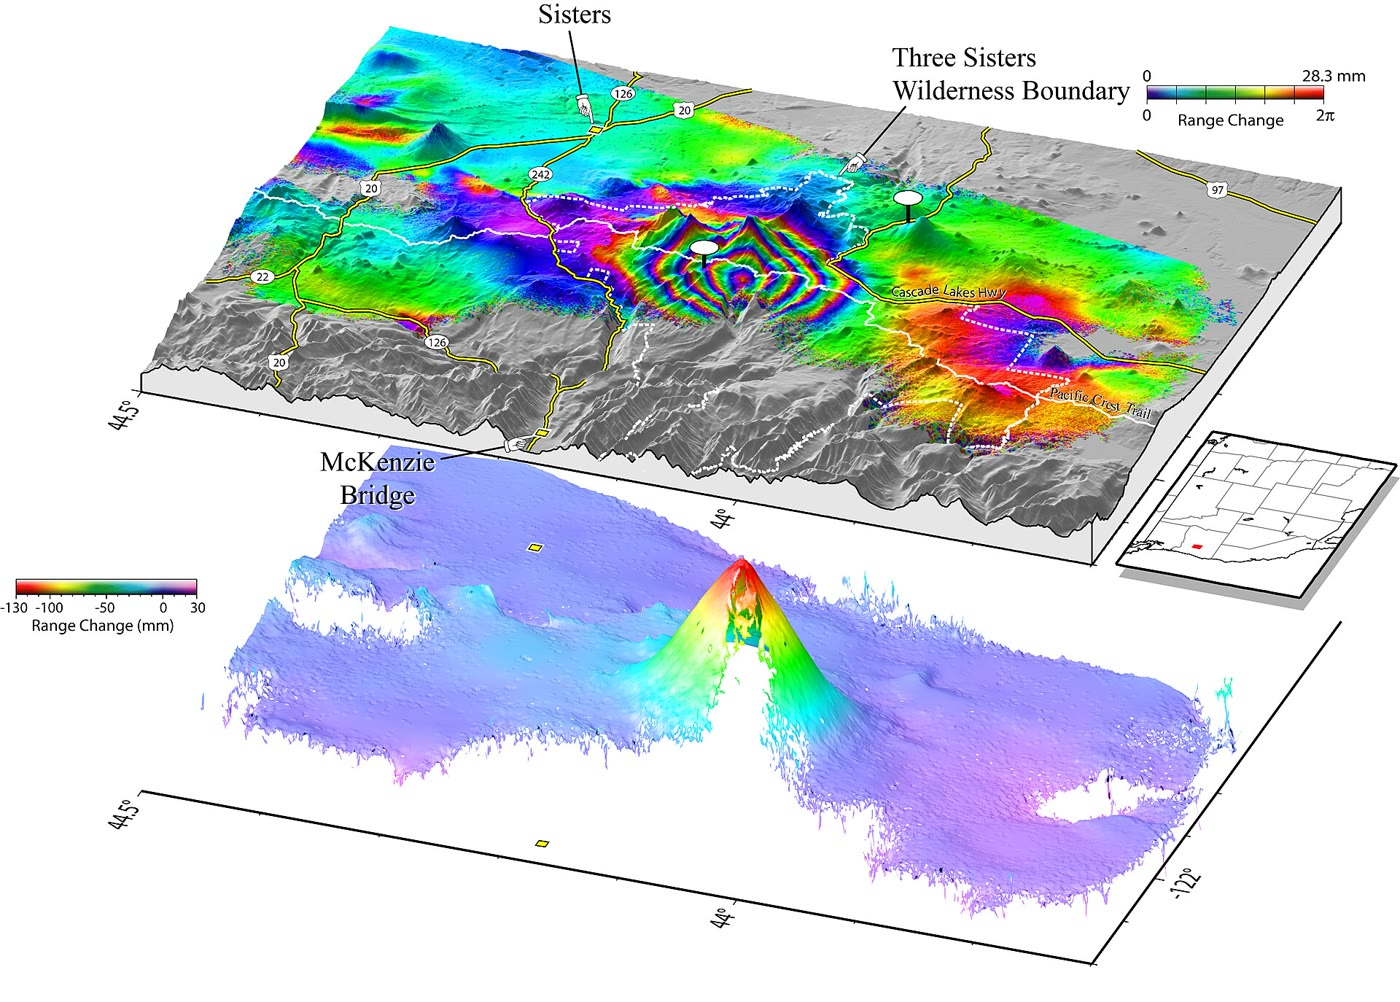
\includegraphics[width=0.86\linewidth]{images/book5/b3-three-sisters-insar.jpg}
\par\smallskip{\small Arriba, el \omterm{def:b3:remote-sensing-gis:insar}{interferograma} del Three Sisters,
centro volcánico, Oregón, 1995--2001, superpuesto al relieve: cada ciclo de
colores equivale a \qty{28.3}{mm} de cambio de distancia, y el ojo de buey de anillos en
el centro marca el levantamiento. Abajo, los mismos datos desenrollados y dibujados como un
relieve: la distancia al satélite se acorta hasta \qty{130}{mm} en el centro. Servicio
Geológico de los Estados Unidos (Wicks y otros, 2002), dominio
público.}\label{fig:b3:remote-sensing-gis:three-sisters}
\end{omfigure}
% ledger: photo:b3-three-sisters-insar, usgs:insar-fs

\begin{inthelab}[Una estación terrena]
\begin{minipage}[t]{0.55\linewidth}\vspace{0pt}
Un satélite de observación registra mucho más de lo que puede enviar mientras pasa
sobre el lugar que fotografía. El radar de un satélite Sentinel-1 puede tomar imágenes
durante hasta media hora de cada órbita y almacena sus datos a bordo, hasta
1410 gigabits; los envía por dos canales de 260 megabits por segundo cada uno, de modo que
vaciar un almacenamiento completo lleva unos 45 minutos. Una estación terrena los recibe:
cuando el satélite asciende sobre el horizonte, la antena gira para apuntarle, lo sigue
a través del cielo y lo suelta al ponerse, mientras los operadores comprueban que el
flujo llega completo. Los datos pasan luego a un centro de procesamiento, donde los ecos
en bruto se convierten en imágenes.
\end{minipage}\hfill
\begin{minipage}[t]{0.42\linewidth}\vspace{0pt}
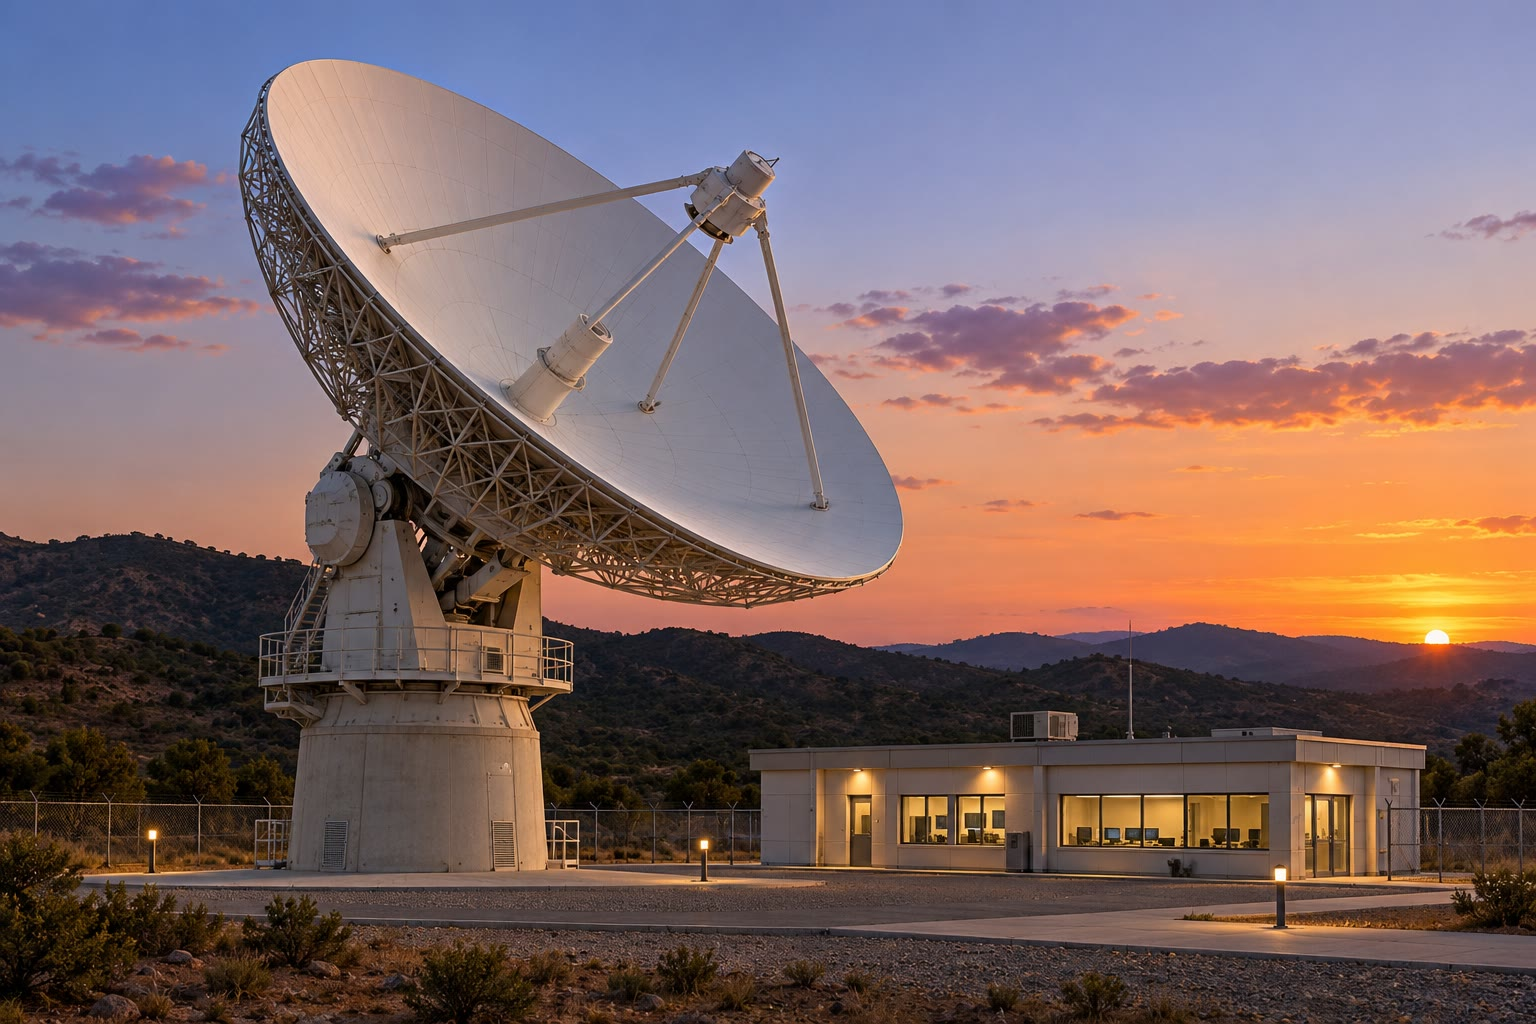
\includegraphics[width=\linewidth]{images/book5/ai/b3-ground-station.jpg}

{\scriptsize Una estación terrena de satélites al atardecer: una gran antena de seguimiento y
su edificio de operaciones (ilustración generada por IA).}
\end{minipage}
\end{inthelab}
% ledger: esa:s1-downlink

\section{Sistemas de información geográfica}\label{sec:b3:remote-sensing-gis:gis}

Las imágenes de los satélites, el modelo de elevaciones del terreno, el
mapa geológico, los pozos y las carreteras son capas de un único sistema de
información geográfica, que las almacena en un marco de coordenadas común y
opera con ellas.

\begin{definition}[Datos ráster y vectoriales]\label{def:b3:remote-sensing-gis:data-models}
Los \emph{datos ráster}\index{datos ráster} representan una capa mediante una malla de
celdas, cada una con un solo valor: una reflectancia, una elevación, una clase.
Los \emph{datos vectoriales}\index{datos vectoriales (SIG)} la representan mediante puntos, líneas
y polígonos definidos por las coordenadas de sus vértices, cada uno con una
fila de atributos en una tabla.
\end{definition}

\begin{omfigure}
\centering
\begin{tikzpicture}[x=0.5cm, y=0.5cm, font=\scriptsize]
\begin{scope}
\draw[black!40] (0,0) rectangle (10,7);
\fill[omSea!50, draw=omDef, thick] (3,4.5) ellipse (1.8 and 1.2);
\draw[omDef, very thick] (4.8,4.5) -- (7,3.5) -- (10,2);
\fill[red!70!black] (7,5.5) circle (0.14); \fill[red!70!black] (2,1.5) circle (0.14);
\node[anchor=south] at (5,7.1) {vectorial};
\node at (3,4.5) {lago};
\node[anchor=south west] at (7.1,5.6) {pozo 1};
\node[anchor=south west] at (2.1,1.6) {pozo 2};
\node[anchor=north east] at (9.9,2.2) {río};
\end{scope}
\begin{scope}[xshift=6.5cm]
\foreach \i/\j in {1/4,2/4,3/4,4/4,2/3,3/3,2/5,3/5} {\fill[omSea!50] (\i,\j) rectangle ++(1,1);}
\foreach \i/\j in {5/4,6/3,7/3,8/2,9/2} {\fill[omDef!70] (\i,\j) rectangle ++(1,1);}
\foreach \i/\j in {7/5,2/1} {\fill[red!70!black] (\i,\j) rectangle ++(1,1);}
\draw[black!30, step=1] (0,0) grid (10,7);
\draw[black!40] (0,0) rectangle (10,7);
\node[anchor=south] at (5,7.1) {ráster};
\end{scope}
\end{tikzpicture}
\par\smallskip{\small El mismo mapa como \omterm{def:b3:remote-sensing-gis:data-models}{datos vectoriales} (izquierda: un polígono, una línea
y dos puntos, exactos en posición, cada uno con sus atributos, y como ráster
\omterm{def:b3:remote-sensing-gis:data-models}{datos ráster} (derecha: un valor por celda, el lago mediante las celdas cuyo centro queda dentro
de él, el río y los pozos mediante las celdas que cruzan). Un ráster es fácil de
calcular, celda a celda; una capa vectorial conserva formas y topología a
cualquier escala.}\label{fig:b3:remote-sensing-gis:raster-vector}
\end{omfigure}

\begin{definition}[Georreferenciación]\label{def:b3:remote-sensing-gis:georef}
La \emph{georreferenciación}\index{georreferenciación} es la asignación de coordenadas de mapa
en una proyección indicada a cada píxel de una imagen o a cada
vértice de un dibujo, normalmente ajustando una transformación a puntos de control en tierra
cuyas posiciones son conocidas en ambos sistemas.
\end{definition}

Para un ráster con el norte hacia arriba en un marco proyectado, la transformación es afín:
la celda de la columna $i$ y la fila $j$ tiene su esquina en $E = E_0 + i\,\Delta$,
$N = N_0 - j\,\Delta$, siendo $\Delta$ el tamaño de celda. Una imagen de satélite se
remuestrea primero en una malla de ese tipo; las capas en proyecciones distintas se
proyectan en una sola antes de combinarlas.

\begin{method}[Pendiente, orientación y sombreado de relieve a partir de un modelo digital de elevaciones]\label{met:b3:remote-sensing-gis:slope}
Sobre una malla de elevaciones $z_{i,j}$ de espaciado $\Delta$ ($i$ hacia el este, $j$
hacia el norte), se estima el gradiente mediante diferencias centrales,
\[
\frac{\partial z}{\partial x} \approx \frac{z_{i+1,j} - z_{i-1,j}}{2\Delta} ,
\qquad
\frac{\partial z}{\partial y} \approx \frac{z_{i,j+1} - z_{i,j-1}}{2\Delta} .
\]
La \emph{pendiente} es $S = \arctan|\nabla z|$; la \emph{orientación} es el
azimut de la máxima pendiente descendente, la dirección de $-\nabla z$, $A =
\operatorname{atan2}(-\partial z/\partial x, -\partial z/\partial y)$
medido en sentido horario desde el norte. El \emph{sombreado de relieve} para una luz procedente del
azimut $A_0$ con ángulo cenital $Z$ es $\cos Z\cos S + \sin Z\sin S
\cos(A_0 - A)$, el coseno del ángulo entre la luz y la normal
al terreno, que se fija en cero donde es negativo.
\end{method}

La diferencia central es exacta para un plano y tiene un error de
$\Delta^2 z'''/6$ en caso contrario; el relieve sombreado de los Varden Hills en el
volumen de primer año se calculó de este modo, iluminado desde el noroeste. Las derivadas
amplifican los errores de la malla: un modelo con escalones entre sus filas los
muestran como franjas en su mapa de pendientes.

\begin{definition}[Álgebra de mapas]\label{def:b3:remote-sensing-gis:map-algebra}
El \emph{álgebra de mapas}\index{algebra de mapas@álgebra de mapas} es el cálculo de una nueva capa ráster
celda a celda a partir de una o más capas de la misma malla: mediante aritmética
(el NDVI a partir de dos bandas), mediante comparación (las celdas más empinadas que
\ang{15}), mediante operaciones lógicas (y, o, no), o a partir de un entorno
de la celda (la pendiente).
\end{definition}

\begin{definition}[Zona de influencia; superposición de capas]\label{def:b3:remote-sensing-gis:operations}
La \emph{zona de influencia}\index{zona de influencia (SIG)} de un elemento a la distancia $d$ es
la región del mapa a menos de $d$ de él. Una
\emph{superposición de capas}\index{superposición de capas (SIG)} combina dos o más capas de la
misma zona en una sola, cada lugar del resultado con los atributos de
todas ellas; la selección de los lugares que cumplen varias condiciones a
la vez es el uso más frecuente.
\end{definition}

\begin{omfigure}
\centering
\begin{tikzpicture}
\begin{groupplot}[group style={group size=2 by 2, horizontal sep=2.0cm, vertical sep=1.5cm},
  width=0.43\linewidth, axis equal image, enlargelimits=false,
  xmin=0, xmax=10, ymin=0, ymax=8,
  tick label style={font=\scriptsize}, label style={font=\small}, title style={font=\small}]
\nextgroupplot[title={(a) pendiente (grados)}, ylabel={norte (km)}, colormap/viridis,
  point meta min=0, point meta max=24, colorbar right,
  colorbar style={width=0.18cm, ytick={0,5,10,15,20}, tick label style={font=\tiny}, axis equal=false}]
\addplot[matrix plot*, mesh/cols=101, point meta=explicit] table[x=x, y=y, meta=slope] {figdata/out/bachelor-3-varden_gis-grid.dat};
\addplot[white, thick] table {figdata/out/shared-region-river.dat};
\nextgroupplot[title={(b) orientación},
  colormap={aspect}{rgb255=(220,20,30) rgb255=(240,200,0) rgb255=(30,170,60) rgb255=(30,90,220) rgb255=(220,20,30)},
  point meta min=0, point meta max=360, colorbar right,
  colorbar style={width=0.18cm, ytick={0,90,180,270,360}, yticklabels={N,E,S,O,N}, tick label style={font=\tiny}, axis equal=false}]
\addplot[matrix plot*, mesh/cols=101, point meta=explicit] table[x=x, y=y, meta=aspect] {figdata/out/bachelor-3-varden_gis-grid.dat};
\addplot[black, thick] table {figdata/out/shared-region-river.dat};
\nextgroupplot[title={(c) dos capas}, xlabel={este (km)}, ylabel={norte (km)},
  colormap={lay}{rgb255=(245,245,245) rgb255=(150,150,150) rgb255=(225,195,140) rgb255=(120,70,20)},
  colormap access=piecewise constant, point meta min=-0.5, point meta max=3.5,
  legend columns=2, legend style={font=\tiny, at={(0.5,-0.3)}, anchor=north, /tikz/every even column/.append style={column sep=4pt}}]
\addplot[matrix plot*, mesh/cols=101, point meta=explicit, forget plot] table[x=x, y=y, meta=layers] {figdata/out/bachelor-3-varden_gis-grid.dat};
\addplot[omDef, thick, forget plot] table {figdata/out/shared-region-river.dat};
\addlegendimage{area legend, fill={rgb,255:red,150;green,150;blue,150}, draw=black!40}
\addlegendentry{más empinado que \ang{15}}
\addlegendimage{area legend, fill={rgb,255:red,225;green,195;blue,140}, draw=black!40}
\addlegendentry{lutita}
\addlegendimage{area legend, fill={rgb,255:red,120;green,70;blue,20}, draw=black!40}
\addlegendentry{ambas condiciones}
\nextgroupplot[title={(d) la superposición}, xlabel={este (km)},
  colormap={cls}{rgb255=(245,245,245) rgb255=(225,195,140) rgb255=(190,150,90) rgb255=(200,20,30)},
  colormap access=piecewise constant, point meta min=-0.5, point meta max=3.5,
  legend columns=2, legend style={font=\tiny, at={(0.5,-0.3)}, anchor=north, /tikz/every even column/.append style={column sep=4pt}}]
\addplot[matrix plot*, mesh/cols=101, point meta=explicit, forget plot] table[x=x, y=y, meta=class] {figdata/out/bachelor-3-varden_gis-grid.dat};
\addplot[omDef, thick, forget plot] table {figdata/out/shared-region-river.dat};
\addplot[black, thin, dashed, unbounded coords=jump] table[x=x, y=y] {figdata/out/bachelor-3-varden_gis-buffer.dat};
\addlegendentry{zona de influencia de \qty{1}{km}}
\addlegendimage{area legend, fill={rgb,255:red,225;green,195;blue,140}, draw=black!40}
\addlegendentry{lutita}
\addlegendimage{area legend, fill={rgb,255:red,190;green,150;blue,90}, draw=black!40}
\addlegendentry{lutita en la zona de influencia}
\addlegendimage{area legend, fill={rgb,255:red,200;green,20;blue,30}, draw=black!40}
\addlegendentry{seleccionado}
\end{groupplot}
\end{tikzpicture}
\par\smallskip{\small Una sesión de SIG sobre los Varden Hills, a partir de su modelo digital de
elevaciones con malla de \qty{100}{m}. (a)~La pendiente, de hasta \ang{23} en las laderas del
valle; (b)~la orientación, la dirección hacia la que mira el terreno, las dos laderas del
río, enfrentadas entre sí; (c)~dos capas, las celdas más empinadas que \ang{15}
y el afloramiento de la lutita jurásica; (d)~su superposición con la
\omterm{def:b3:remote-sensing-gis:operations}{zona de influencia} de \qty{1}{km} del río (a trazos): los \qty{0.32}{km^2} de lutita empinada
sobre el río, una primera criba del terreno que puede
deslizarse.}\label{fig:b3:remote-sensing-gis:varden}
\end{omfigure}

La figura de arriba recorre toda la cadena: el \omterm{def:b3:remote-sensing-gis:map-algebra}{álgebra de mapas} sobre la malla de elevaciones
da la pendiente y la orientación; una comparación convierte la pendiente en una capa
de celdas empinadas; el mapa geológico aporta la lutita; la \omterm{def:b3:remote-sensing-gis:operations}{zona de influencia}
del río da una tercera capa; su intersección, una superposición con la
\emph{y} lógica, deja 32 celdas de las 8181. La respuesta solo es tan buena como
las capas: en una malla más gruesa las pendientes salen más suaves y pasan menos celdas.

\begin{definition}[Clasificación supervisada; matriz de confusión]\label{def:b3:remote-sensing-gis:classification}
Una \emph{clasificación supervisada}\index{clasificación supervisada}
asigna cada píxel de una imagen a una de un conjunto de clases, a partir de reglas o
estadísticas aprendidas sobre píxeles de entrenamiento cuya clase se conoce en el terreno.
Su \emph{matriz de confusión}\index{matriz de confusión} cuenta, para un conjunto
separado de píxeles de referencia, cuántos de cada clase verdadera se asignaron a cada
clase: $n_{ij}$ píxeles clasificados como $i$ pertenecen en realidad a $j$.
\end{definition}

La diagonal recoge los píxeles clasificados correctamente. Con $N$ píxeles de referencia,
la \emph{exactitud global} es $\sum_i n_{ii}/N$. La \emph{exactitud del usuario}
de una clase, $n_{ii}$ sobre su total de fila, es la probabilidad de que un
píxel que el mapa llama $i$ sea $i$; su \emph{exactitud del productor}, $n_{ii}$
sobre su total de columna, la probabilidad de que un $i$ verdadero se haya cartografiado como $i$. El
coeficiente \emph{kappa} compara la exactitud global $p_o$ con la
exactitud $p_e = \sum_i (\text{row}_i)(\text{col}_i)/N^2$ que alcanzaría una
asignación aleatoria con los mismos totales: $\kappa = (p_o - p_e)/(1 -
p_e)$.

\begin{center}
\small
\begin{tabular}{l|ccc|c}
\hline
clasificado \textbackslash{} referencia & agua & bosque & roca desnuda & total \\
\hline
agua & 45 & 2 & 0 & 47 \\
bosque & 3 & 38 & 7 & 48 \\
roca desnuda & 0 & 5 & 30 & 35 \\
\hline
total & 48 & 45 & 37 & 130 \\
\hline
\end{tabular}
\end{center}

En este ejemplo inventado, 113 de 130 píxeles son correctos, una exactitud global
de \qty{86.9}{\percent}. El bosque tiene una exactitud del usuario de
$38/48 = \qty{79}{\percent}$ pero una exactitud del productor de $38/45 =
\qty{84}{\percent}$: siete píxeles de roca desnuda, quizá en sombra, se
llamaron bosque. Una asignación aleatoria alcanzaría $p_e = 0.338$, y $\kappa =
0.80$.

\section{Ejercicios}

\begin{exercise}[$\star$]\label{exo:b3:remote-sensing-gis:1}
Un campo tiene reflectancias de 0.06 en la banda roja y 0.42 en la
banda del infrarrojo cercano de un sensor de imágenes; un campo arado junto a él, 0.21 y
0.28. Calcúlese el NDVI de ambos y explíquese qué sugiere cada valor.
\end{exercise}

\begin{exercise}[$\star$]\label{exo:b3:remote-sensing-gis:2}
El sensor Landsat~8 cubre una franja de \qty{185}{km} de ancho con píxeles de
\qty{30}{m}, y su banda pancromática con píxeles de \qty{15}{m}. (a)~¿Cuántos
píxeles contiene una línea a través de la franja en cada caso? (b)~¿Cuántos niveles
dan 12 bits, y 8 bits? (c)~¿Cuál es el \omterm{def:b3:remote-sensing-gis:resolutions}{tiempo de revisita} de Landsat~8
por sí solo, y el de Landsat~8 y 9 juntos?
\end{exercise}

\begin{exercise}[$\star$]\label{exo:b3:remote-sensing-gis:3}
(a)~En un \omterm{def:b3:remote-sensing-gis:insar}{interferograma} de Sentinel-1 ($\lambda = \qty{5.55}{cm}$) de una
cuenca en subsidencia, seis franjas separan el borde estable del centro.
¿Cuál es el cambio de la \omterm{def:b3:remote-sensing-gis:insar}{línea de visión} en el centro? (b)~¿Cuánto valdría una
franja para un satélite más antiguo de longitud de onda \qty{5.66}{cm}?
\end{exercise}

\begin{exercise}[$\star$]\label{exo:b3:remote-sensing-gis:4}
Un altímetro láser está a \qty{500}{km} sobre el suelo. (a)~¿Cuánto tarda en volver
un pulso? (b)~Si cada fotón se cronometra con \qty{800}{ps}, ¿qué precisión tiene
una medida de distancia?
\end{exercise}

\begin{exercise}[$\star\star$]\label{exo:b3:remote-sensing-gis:5}
Un píxel de la banda~10 de Landsat~8 (tómese $\lambda = \qty{10.9}{\micro\metre}$)
tiene, tras la \omterm{def:b3:remote-sensing-gis:atm-correction}{corrección atmosférica}, una radiancia espectral de
\qty{9.0}{W.m^{-2}.sr^{-1}.\micro\metre^{-1}}. (a)~Calcúlese la
\omterm{def:b3:remote-sensing-gis:brightness}{temperatura de brillo}. (b)~La superficie es un prado de emisividad 0.98: ¿cuál es
su temperatura cinética?
\end{exercise}

\begin{exercise}[$\star\star$]\label{exo:b3:remote-sensing-gis:6}
El radar Sentinel-1 vuela a \qty{693}{km} de altura con una antena de \qty{12.3}{m}
de largo a $\lambda = \qty{5.55}{cm}$. (a)~Despreciando la curvatura de la
Tierra, calcúlese la distancia oblicua a un punto visto con una incidencia de
\ang{35}. (b)~¿Qué resolución en azimut daría una antena real de esa longitud
allí, y qué da la apertura sintética? (c)~¿Cuánto mide la
apertura sintética?
\end{exercise}

\begin{exercise}[$\star\star$]\label{exo:b3:remote-sensing-gis:7}
Una ventana de $3\times3$ de un modelo digital de elevaciones con celdas de \qty{30}{m}
da, con el norte arriba,
\[
\begin{matrix} 412 & 418 & 425 \\ 405 & 410 & 418 \\ 398 & 401 & 409 \end{matrix}
\qquad (\unit{m}).
\]
Por diferencias centrales en la celda central, calcúlense la pendiente, la orientación
y el sombreado para una luz desde el noroeste, a \ang{45} sobre el
horizonte.
\end{exercise}

\begin{exercise}[$\star\star$]\label{exo:b3:remote-sensing-gis:8}
Un mapa de cubiertas del suelo se contrasta con 160 píxeles de referencia (filas: el mapa;
columnas: la realidad; clases agua, bosque, cultivos, pueblo):
\[
\begin{pmatrix} 48 & 3 & 1 & 0 \\ 4 & 37 & 6 & 1 \\ 2 & 5 & 29 & 2 \\ 0 & 1 & 2 & 19 \end{pmatrix} .
\]
Calcúlense la exactitud global, las exactitudes del usuario y del productor de cada
clase, y kappa. ¿Qué clase se omite con más frecuencia?
\end{exercise}

\begin{exercise}[$\star\star$]\label{exo:b3:remote-sensing-gis:9}
Un píxel térmico de \qty{100}{m} contiene una colada de lava reciente a \qty{1443}{K}
que cubre el \qty{4}{\percent} de él; el resto es suelo a \qty{290}{K}; considérense
ambos como cuerpos negros. (a)~Calcúlese la \omterm{def:b3:remote-sensing-gis:brightness}{temperatura de brillo} del píxel
a \qty{10.9}{\micro\metre} y compárese con la temperatura media.
(b)~Calcúlese la razón de las radiancias de cuerpo negro de la lava y del
suelo a \qty{2.2}{\micro\metre}, y la \omterm{def:b3:remote-sensing-gis:brightness}{temperatura de brillo} del
píxel en esa banda. ¿Qué banda detecta mejor la lava?
\end{exercise}

\begin{exercise}[$\star\star\star$]\label{exo:b3:remote-sensing-gis:10}
Se construyen dos \omterm{def:b3:remote-sensing-gis:insar}{interferogramas} de la misma deformación a partir de dos pasadas, una
con el satélite al este del terreno y otra con él al oeste,
ambas con un ángulo de incidencia de \ang{35}. En un punto, la
\omterm{def:b3:remote-sensing-gis:insar}{línea de visión} se acorta \qty{64}{mm} en el primero y \qty{38}{mm} en el
segundo. Suponiendo que no hay movimiento norte--sur, calcúlense el desplazamiento vertical y el
desplazamiento hacia el este. ¿Por qué no basta con una sola pasada?
\end{exercise}

\begin{exercise}[$\star\star\star$]\label{exo:b3:remote-sensing-gis:11}
El desenrollado falla donde la fase salta más de $\pi$ entre
píxeles vecinos. (a)~Demuéstrese que la \omterm{def:b3:remote-sensing-gis:insar}{línea de visión} debe cambiar menos de $\lambda/4$ de un
píxel al siguiente, \qty{13.9}{mm} para
Sentinel-1. (b)~Para una fuente de Mogi a $z_0 = \qty{4}{km}$ con $\Delta V =
\qty{e7}{m^3}$ y $\nu = 0.25$, vista en vertical, demuéstrese que el
gradiente más pronunciado de $u_z$ está en $r = z_0/2$ y calcúlese. (c)~¿Cuál es el
mayor tamaño de píxel que mantiene resolubles las franjas?
\end{exercise}

\begin{exercise}[$\star\star\star$]\label{exo:b3:remote-sensing-gis:12}
(a)~Demuéstrese que el NDVI está entre $-1$ y $+1$ para reflectancias no negativas,
y que no cambia cuando ambas reflectancias se multiplican
por un mismo factor. (b)~La hierba tiene reflectancias de 0.051 (rojo)
y 0.502 (infrarrojo cercano). Una imagen sin corregir añade una radiancia de trayectoria
equivalente a 0.03 en el rojo y 0.01 en el infrarrojo cercano. Calcúlese el
NDVI con y sin ella. (c)~¿Qué implica eso para un mapa del NDVI
elaborado con imágenes sin corregir en un día de bruma?
\end{exercise}

\section{Problema: un flanco en hinchamiento en el monte Halvren}

\begin{problem}[{Problema de fin de semana --- vegetación, calor e interferograma radar
de un volcán ficticio}]
\label{pb:b3:remote-sensing-gis:1}
El monte Halvren, un volcán ficticio, ha emitido coladas de lava en 1890, 1960
y 2005 sobre sus flancos boscosos. Un campo de fumarolas humea en su cima.
Se dan a continuación datos de satélite de un año reciente.

\medskip\noindent\textbf{Parte I --- Vegetación sobre las coladas de lava.} Reflectancias corregidas
en las bandas del rojo y del infrarrojo cercano:
\begin{center}
\small
\begin{tabular}{lcccc}
\hline
superficie & bosque & colada de 1890 & colada de 1960 & colada de 2005 \\
\hline
rojo & 0.04 & 0.07 & 0.11 & 0.12 \\
infrarrojo cercano & 0.38 & 0.30 & 0.21 & 0.14 \\
\hline
\end{tabular}
\end{center}
\begin{enumerate}
\item Calcúlese el NDVI de las cuatro superficies.
\item Ordénense las coladas según la recuperación de su vegetación. ¿Coincide el orden
  con el de sus edades?
\item ¿Por qué el NDVI de la colada de 2005 no es cero, aunque casi
  nada crece sobre ella?
\item ¿Por qué el NDVI es más fiable que la reflectancia en el infrarrojo cercano
  por sí sola en los flancos empinados e irregularmente iluminados de un volcán?
\end{enumerate}

\medskip\noindent\textbf{Parte II --- El campo de fumarolas.} En la banda térmica
(tómese $\lambda = \qty{10.9}{\micro\metre}$) la radiancia corregida de
un píxel de \qty{100}{m} de la meseta de la cima alejado de las fumarolas es
\qty{8.40}{W.m^{-2}.sr^{-1}.\micro\metre^{-1}}, y la del píxel sobre
el campo de fumarolas \qty{9.95}{W.m^{-2}.sr^{-1}.\micro\metre^{-1}}.
\begin{enumerate}[resume]
\item Calcúlense las \omterm{def:b3:remote-sensing-gis:brightness}{temperaturas de brillo} de los dos píxeles.
\item La roca de la meseta tiene una emisividad de 0.97. ¿Cuál es su temperatura
  cinética?
\item Las bocas de las fumarolas y el suelo caliente que las rodea están a
  \qty{370}{K}. Considerándolos, junto con el resto del píxel, como cuerpos negros,
  quedando el resto con la radiancia de la meseta, ¿qué fracción del píxel
  cubren, y qué superficie?
\item ¿Por qué la temperatura media del píxel, ponderada por área, queda por debajo
  de su \omterm{def:b3:remote-sensing-gis:brightness}{temperatura de brillo}?
\end{enumerate}

\medskip\noindent\textbf{Parte III --- El interferograma.} Dos imágenes de Sentinel-1
($\lambda = \qty{5.55}{cm}$, incidencia \ang{35}, satélite al
este) tomadas con 48 días de diferencia muestran un patrón concéntrico en el flanco este. Desde una
zona estable hasta el centro del patrón se cuentan cinco franjas completas y
cuatro décimas de una sexta, todas ellas en el sentido del movimiento hacia el
satélite.
\begin{enumerate}[resume]
\item ¿Por qué deben tomarse dos imágenes casi desde la misma posición, y cuántos
  ciclos orbitales de un mismo satélite las separan?
\item Calcúlese el cambio de la \omterm{def:b3:remote-sensing-gis:insar}{línea de visión} en el centro.
\item En el centro el terreno se mueve solo verticalmente. Calcúlese el levantamiento
  allí.
\item Explíquese por qué el patrón no es circular y en qué lado, este u oeste,
  se concentran las franjas.
\item A lo largo de la línea norte--sur que pasa por el centro, el cambio de la
  \omterm{def:b3:remote-sensing-gis:insar}{línea de visión} se reduce a la mitad de su valor central a \qty{3.4}{km} del
  centro. ¿Por qué usar esa línea y qué profundidad da para una fuente
  de Mogi?
\item ¿Cuántas franjas separan el centro de ese punto a media altura?
\item El vapor de agua del aire puede retrasar las ondas de radar de forma distinta en las
  dos fechas y dibujar franjas propias. ¿Cómo ayudaría un segundo \omterm{def:b3:remote-sensing-gis:insar}{interferograma},
  de otro par de fechas, a distinguir entre ambas?
\end{enumerate}

\medskip\noindent\textbf{Parte IV --- El volumen.} Tómese $\nu = 0.25$.
\begin{enumerate}[resume]
\item A partir de $u_z(0) = (1 - \nu)\Delta V/(\pi z_0^2)$, calcúlese la variación de volumen
  de la fuente.
\item Exprésese como tasa media por día y por año a lo largo de los 48 días.
\item Calcúlese el mayor desplazamiento horizontal y dónde se produce.
\item Si el reservorio fuera una esfera de radio $z_0/3$, ¿cuál sería su
  volumen, y qué fracción de él representa la variación?
\item El tamaño finito de una esfera de radio $z_0/3$ modifica el levantamiento en
  unos \qty{3}{\percent}. ¿Cambia la respuesta a la pregunta~16
  de forma apreciable, dada la precisión del recuento de franjas?
\item ¿Qué otra observación, de las partes I y II o tomada sobre el terreno,
  respaldaría la interpretación de un reservorio en llenado?
\item Dése la variación de volumen del reservorio bajo el monte Halvren, en
  millones de metros cúbicos, con dos cifras significativas.
\end{enumerate}
\end{problem}
% ledger: nasa:ndvi, esa:s1-sar, esa:s1-orbit, esa:s1-iw, dmodels:mogi, dmodels:mogi-radial, const:h, const:c, const:kB
